\chapter{GÉNÉRALITÉS ET ÉTUDE PRÉALABLE}

\section{Introduction partielle}
La localisation, le repérage des pairs ou la navigation ont toujours posé des défis. À différentes époques, les solutions de localisation ont tiré parti des technologies de pointe disponibles: détermination de la position des étoiles \cite{polaris}, utilisation de phares maritimes (depuis l'Antiquité jusqu'à nos jours) et aéronautiques depuis les années 1920 \cite{michael_brian_schiffer_electric_2005}. Bien que la navigation ait longtemps été basée sur la référence à des points connus (villes, étoiles, phares), elle a progressivement cherché à améliorer sa précision. Deux approches ont émergé: la triangulation, où l'utilisateur mesure les angles par rapport aux points de référence pour déduire sa position (notamment grâce au sextant au XVIIe siècle), et la navigation à l'estime, où l'utilisateur part de sa position initiale puis suit ses mouvements en utilisant des instruments de mesure tels que des compas, une méthode employée depuis le XVe siècle et popularisée par Christophe Colomb lors de sa découverte des Amériques \cite{frederic_chapin_lane_venice_1973}. Ce n'est qu'à la fin du XXe siècle que les systèmes de trilatération (d'abord terrestres, puis par satellites avec le GPS) ont pris le dessus en raison de leur précision et de leur couverture \cite{p_daly_navstar_nodate}.

\section{Les moyens de localisation actuels à grande échelle}

\subsection{Les systèmes de localisation par réseaux terrestres}
Aujourd’hui, de nombreux réseaux cellulaires ou sans fil existent. Ces réseaux communiquent avec les équipements mobiles par radio. Le premier système de ce type est le système LORAN C dans les années 1960. Ensuite, les réseaux comme le GSM et l’UMTS ou le réseau de TNT (Télédiffusion Numérique Terrestre) sont apparus pour arelayer le système LORAN C \cite{frederic_evennou_techniques_2007}.

\subsubsection{Le système LORAN C}

LORAN est un acronyme de Long Range Navigation, l’évolution du concept original de LORAN pour répondre aux exigences opérationnelles pour une plus grande précision et une plus grande portée de service a donné lieu au développement de trois systèmes connexes : LORAN A, LORAN B et LORAN C.\\

Loran C est basé sur la mesure de la différence de temps d’arrivée des ondes provenant de deux stations terrestres différentes. Le lieu géométrique représenté par cette différence de temps est une hyperbole. Pour fonctionner, il est nécessaire de connaître la position de chacune des stations terrestres et les stations terrestres doivent être synchronisées entre elles afin de comparer les instants d’arrivée des différents signaux \cite{frederic_evennou_techniques_2007}.\\

Dans le cadre de LORAN, il y a une des stations qui sert de référence à toutes  (appelée station maître), les autres stations sont dites esclaves.
\begin{figure}[H]
	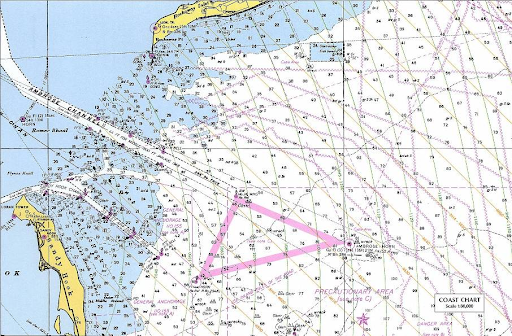
\includegraphics[width=\textwidth]{carteloran}
	\caption{Carte d’une station de base LORAN}
\end{figure}

Le processus de localisation se déroule de la manière suivante : le dispositif mobile calcule la variation de temps entre l'arrivée des signaux de la station maître et d'une station esclave, ce qui génère une ligne de position. Une deuxième ligne de position est obtenue en mesurant une autre variation de temps entre la station principale et une deuxième station secondaire. La convergence de ces deux approches aboutit à la détermination de la position du dispositif mobile \cite{frederic_evennou_techniques_2007}.\\

La navigation s'appuie sur des cartes préétablies. Le récepteur LORAN n'effectue pas de calculs de position par lui-même. Les cartes marines, telles que celle illustrée à la Figure 1.1, représentent les différents décalages observables. L'intersection des diverses ligne de position donne lieu à une approximation de la position du navire. Dans les récepteurs modernes, les valeurs affichées ne sont plus les variations de temps, mais plutôt les coordonnées de latitude et de longitude correspondantes, Les précisions données pour ce système de navigation sont de l’ordre de 500 m. Pour des applications de navigation maritime, cette précision était suffisante avant l’arrivée du GPS \cite{frederic_evennou_techniques_2007}.

\subsubsection{La localisation par réseau GSM}
La localisation par GSM consiste à positionner un terminal GSM en se basant sur des informations liées aux antennes GSM auxquelles le terminal est connecté. La précision de la géolocalisation par GSM varie généralement de 200 mètres à plusieurs kilomètres, en fonction de la localisation du terminal, qu'il soit en milieu urbain ou rural.\\

\noindent Les trois technologies de géolocalisation distinctes utilisées par le GSM sont :

\begin{itemize}
	\item Le différentiel temps dit EOTD (Enhanced Observed Time Difference) : Le téléphone mobile émet un signal vers les stations mobiles environnantes, celle qui est la plus proche lui renvoie ce signal. Le temps écoulé entre l’émission et la réception de cette onde est analysée par un serveur externe qui calculera la localisation du téléphone portable dans le réseau.
	
	\item Le système de l’identification de cellule ou Cell ID (Cellule IDentify) : Le système de l’identification par cellule est la technique de géolocalisation la plus simple et la moins couteuse. Lorsque l’utilisateur se trouve dans une zone couverte par le réseau, il est localisé grâce à l’identification de la cellule à laquelle appartient l’antenne et par laquelle la communication est transmise.
	
	\item La triangulation : Le système de la triangulation repose sur le traitement croisé des informations provenant en permanence de trois relais émetteur et récepteur qui changent au fur et à mesure que l’antenne hertzienne utilisée par le portable de l’usager se déplace.
\end{itemize}

\subsubsection{La géolocalisation par Wi-Fi} 
La géolocalisation par Wi-Fi constitue une solution adaptée tant pour le positionnement à l'intérieur que l'extérieur des bâtiments.
De manière similaire à la méthode Cell ID utilisée pour la géolocalisation sur un réseau GSM, un terminal Wi-Fi peut se localiser en se basant sur les identifiants de bornes Wi-Fi (adresses MAC) qu'il détecte. Des bases de données répertoriant de nombreuses bornes Wi-Fi ainsi que leurs positions géographiques existent. Ces bases de données peuvent être la propriété d'entreprises privées ou être mises à disposition gratuitement par des sociétés.

\subsubsection{Limites des systèmes de localisation par réseaux terrestres }
 
Ces systèmes terrestres possèdent une portée limitée, dans la mesure où ils supposent une surface de localisation plane, ce qui n’est pas le cas de la Terre. De plus, le signal envoyé est affaibli dans l’air, et peut même être dégradé par des obstacles ou par les conditions météorologiques. Malgré tout, ces systèmes sont toujours opérationnels, pour des applications précises comme l’aéronautique, ou en complément des systèmes satellitaires \cite{frederic_evennou_techniques_2007}.

\subsection{ Les systèmes de localisation satellitaires}
L'émergence d'un système mondial de localisation s'est manifestée avec les avancées dans la conquête spatiale dans les années 1960. Les États-Unis ont introduit le tout premier système de positionnement par satellite en 1964, baptisé TRANSIT \cite{w_guier_and_g_weiffenbach_genesis_1997}. Ce système utilisait l'effet Doppler subi par le signal émis, lequel renfermait des informations précises sur la position du satellite émetteur, appelée éphéméride. Cette méthode permettait de se localiser dans le cadre du référentiel géodésique terrestre. Répondant aux exigences militaires, les États-Unis ont entrepris dans les années 1970 le développement d'une solution plus précise. \\

En effet, le système TRANSIT était entravé par les limitations imposées par la propagation du signal satellite dans l'atmosphère, incluant les affaiblissements dus à la troposphère et la dispersion des fréquences dans l'ionosphère. Ces facteurs ne permettaient qu'une précision de l'ordre de quelques centaines de mètres.

\subsubsection{La localisation par GPS}
Le GPS représente le système de localisation le plus répandu parmi les systèmes mondiaux de positionnement par satellites. Il est entièrement opérationnel et accessible partout. En effet, grâce au GPS, il est possible d'obtenir instantanément la localisation précise de n'importe quel endroit sur la planète.

Le système GPS englobe une constellation composée d'au moins 24 satellites tournant autour de la Terre suivant six orbites différentes. Chacune de ces orbites est inclinée à un angle de 55 degrés par rapport à l'équateur terrestre. Les orbites sont réparties de manière à être séparées de 60 degrés les unes des autres, garantissant ainsi une couverture de 260 degrés sur l'ensemble de la planète. Chaque orbite possède un rayon de 26 560 km. Ces orbites sont configurées de manière que les satellites effectuent une révolution complète autour de la Terre en l'espace d'une journée sidérale. Les quatre satellites se trouvant sur une orbite ne se trouvent pas à équidistance sur cette dernière. Deux des satellites sont espacés d'un angle variant entre 30,0 et 32,1 degrés. Les deux autres satellites forment un angle compris entre 92,28 et 130,98 degrés par rapport aux trois autres. Cette configuration a été mise en place afin de minimiser les effets en cas de dysfonctionnement d'un des satellites. Théoriquement, un récepteur GPS devrait être en mesure de capter entre 4 et 11 satellites depuis n'importe quel point de la surface terrestre \cite{frederic_evennou_techniques_2007}.

\subsubsection{GLONASS }
GLONASS est un système russe de navigation par satellite fonctionnant dans le cadre d'un service de radionavigation par satellite. Il constitue une alternative au système de positionnement global et est le deuxième système de navigation en service avec une couverture mondiale et une précision comparable \cite{bernhard_hofmann_wellenhof_gnss}.\\

Le système GLONASS repose sur une constellation de 24 satellites en mouvement, répartis sur 3 plans orbitaux et situés à une altitude de 19 100 km. Le programme GLONASS a été initié en 1982 et a été déclaré opérationnel à part entière en 1993 par les autorités russes. Toutefois, en raison de contraintes financières rencontrées par l'Union Soviétique et de la relativement courte durée de vie des satellites (de 2 à 3 ans), la constellation a progressivement subi une détérioration. À l'heure actuelle, le système fonctionne en mode réduit avec seulement sept satellites opérationnels. Ce système trouve son application en géodésie, grâce à l'utilisation de mesures de phase.\\

L’intérêt de ce système de navigation réside en sa robustesse aux interférences. Chaque satellite émet sur sa propre fréquence (FDMA). Les satellites balaient une plus grande région du globe notamment les regions nord du fait des caractéristiques de la constellation de satellites et du plan d’inclinaison. Le principal défaut du système est qu’il n’est guère entretenu. L’entretien des satellites est très onéreux et du fait que les autorités russes manquent de moyens financiers, aujourd’hui seulement sept satellites sur les vingt quatre sont opérationnels \cite{frederic_evennou_techniques_2007}.

\subsubsection{Galileo}
Galileo est destiné à être un GNSS civil de l'UE qui permet à tous les utilisateurs d'y accéder. À l'origine, le GPS réservait le signal de la plus haute qualité à un usage militaire, et le signal disponible pour un usage civil était intentionnellement dégradé (disponibilité sélective). Cette situation a changé lorsque le président Bill Clinton a signé une directive politique en 1996 pour désactiver la disponibilité sélective. Depuis mai 2000, le même signal de précision est fourni aux civils et aux militaires \cite{bernhard_hofmann_wellenhof_gnss}.\\

Sur le plan conceptuel, GALILEO ne différera pas de manière significative du GPS. Il reposera sur une constellation de 30 satellites, chacun ayant une masse d'environ 700 kg. Ces satellites seront agencés en trois plans orbitaux inclinés à un angle de 56 degrés par rapport à l'équateur, évoluant à une altitude de 23 500 km. Chaque satellite effectuera une rotation complète autour de la Terre en environ 14 heures. La gestion de la constellation sera assurée par un réseau global de stations terrestres \cite{bernhard_hofmann_wellenhof_gnss}.

\section{Localisation d’un terminal par GPS}
Le GPS est un système satellitaire qui est le plus populaire parmi les systèmes de positionnement mondial par satellites qui produit des informations en continu aux récepteurs GPS. Dans la vie quotidienne, les récepteurs GPS sont intégrés à de nombreux objets tels que les téléphones portables, les appareils photo et les automobiles. Ils sont également utilisés dans des dispositifs plus spécialisés tels que les robots d'exploration et les GPS de randonnée.\\

Il est constitué de trois parties distinctes nommées segments qui sont le segment spatial, le segment de contrôle et le segment utilisateur.

\begin{itemize}[label=-]
\item \textit{Le segment spatial}
\end{itemize}


Le segment spatial, composé des satellites, constitue le cœur du système GPS. Ces satellites forment une constellation en orbite autour de la Terre, évoluant à une altitude supérieure à 19 000 km. Cette altitude élevée permet une couverture étendue des signaux sur une large zone. Les orbites des satellites sont organisées de manière à ce qu'à tout moment, un récepteur GPS puisse capter les signaux d'au moins trois satellites simultanément.\\

Les satellites envoient des signaux radio à faible puissance et sur des fréquences différentes. Ces signaux sont capables de traverser des matériaux tels que le plastique, le verre et les nuages, mais ils sont bloqués par des objets denses ou solides tels que les bâtiments et les montagnes. Chaque satellite émet un code unique, ce qui permet aux récepteurs GPS d'identifier et de différencier les signaux émanant de chaque satellite.

\begin{itemize}[label=-]
\item \textit{Le segment de contrôle : }
\end{itemize}

Il assure la supervision des satellites GPS, en les suivant et en leur fournissant des ajustements au niveau du temps et des orbites. Ce segment comprend cinq stations de contrôle réparties dans le monde, chacune étant située à différents endroits autour de la Terre. Parmi ces cinq stations, quatre sont automatisées et sont chargées de la surveillance des satellites, tandis qu'une station principale est dédiée au contrôle global. Les stations automatiques reçoivent des données des satellites et transmettent ces informations à la station de contrôle principale. Cette dernière procède à la mise à jour et à la correction des données reçues, puis renvoie ces informations aux satellites à l'aide de deux antennes situées sur deux autres.

\begin{itemize}[label=-]
	\item \textit{Le segment utilisateur}
\end{itemize}

Le segment utilisateur comprend les utilisateurs militaires et civils qui reçoivent et utilisent les informations émanant des satellites via un récepteur GPS. Ce segment englobe diverses catégories d'utilisateurs, notamment les forces de police, la gendarmerie, les militaires (armée de terre, marine, etc.) dans le domaine militaire. Dans le domaine civil, ce segment rassemble les pilotes, les navigateurs maritimes, les pêcheurs, les sportifs, les chasseurs, les conducteurs d'engins, les randonneurs, et bien d'autres.

\subsection{La trilatération}

Afin de fonctionner correctement, le récepteur GPS doit acquérir deux informations fondamentales : la distance entre lui et les satellites ainsi que les positions exactes de ces satellites. Après avoir capté les signaux émis par les satellites, le récepteur mesure le temps nécessaire à la propagation de ces ondes, ce qui lui permet de calculer la distance qui le sépare de chaque satellite. Cette opération est ensuite répétée pour les autres satellites en vue.
Une fois que les distances entre le récepteur et les satellites sont connues, il devient possible de calculer et de déterminer la position grâce à une technique de triangulation. Pour obtenir une position en deux dimensions, trois satellites sont nécessaires, tandis que pour une position en trois dimensions, quatre satellites sont requis.

\begin{figure}[H]
	
\includegraphics[width=\textwidth]{trilateration1d}
	\caption{Principe du GPS dans un espace 1-D}
\end{figure}

Lorsqu'un équipement U (qu'il s'agisse d'un satellite ou d'un appareil mobile) effectue une mesure et évalue la distance qui le sépare du satellite S1, cela engendre deux positions potentielles pour U : soit à gauche de S1, soit à sa droite. Pour lever cette incertitude de position, l'utilisation d'un second satellite devient nécessaire. Dans ce scénario, c'est le satellite S2 qui intervient pour résoudre cette ambiguïté. Lorsque S2 évalue la distance entre lui et l'équipement U à x2, cela permet de déterminer la seule position plausible, comme illustrée par U sur la figure 1.2.\\

Le processus de détermination de la position d'un équipement dans un espace à deux ou trois dimensions suit une logique similaire à celle utilisée pour la localisation en une dimension. Dans cette configuration, l'obligation est d'avoir trois satellites à partir desquels trois distances sont mesurées. Le lieu géométrique associé à une distance spécifique par rapport à un point fixe est un cercle dans le cas bidimensionnel. La figure 1.3 démontre que deux satellites conduisent à l'estimation de deux positions dans l'espace. Cependant, l'introduction d'un troisième cercle est nécessaire pour déterminer la position unique de l'utilisateur.

\begin{figure}[H]
	\centering
	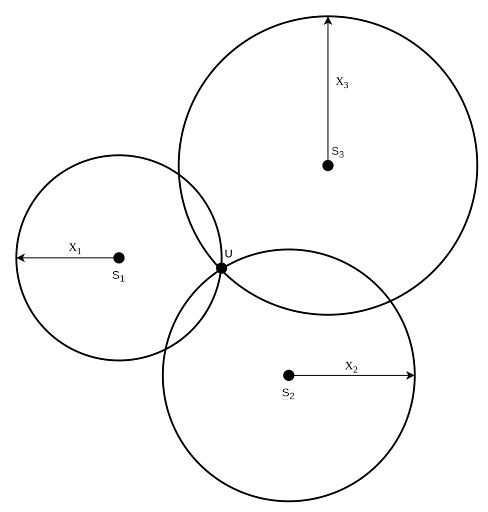
\includegraphics[width=4.48in, height=4.71in]{gps2d}
	\caption{Principe du GPS dans un espace 2-D}
\end{figure}

De la même manière, on aboutit à la nécessité de disposer de quatre satellites pour parvenir à une localisation dans un espace à trois dimensions. Dans cet espace, le lieu géométrique correspondant est une sphère dont le rayon est la distance entre le satellite et l'utilisateur. On sait que l'intersection de deux sphères est un cercle. L'intersection de ce cercle avec une sphère génère deux points dans l'espace, et la troisième sphère détermine quelle position parmi les deux est occupée par l'équipement mobile.

\section{ÉTUDE PRÉALABLE}
Il existe aujourd’hui toute une panoplie des applications utilisant la géolocalisation et pouvant permettre à une personne en danger d’être localisé et de bénéficier d’une assistance. Dans cette partie, nous allons présenter ces applications, ensuite, nous allons établir une étude critique et enfin, nous allons proposer des pistes de solution qui nous permettront d’avoir plus de lumière avant de passer à la conception de notre solution.

\subsection{Étude de l’existant}
\subsubsection{ICE GeoAlert}
\begin{figure}[H]
	\centering
	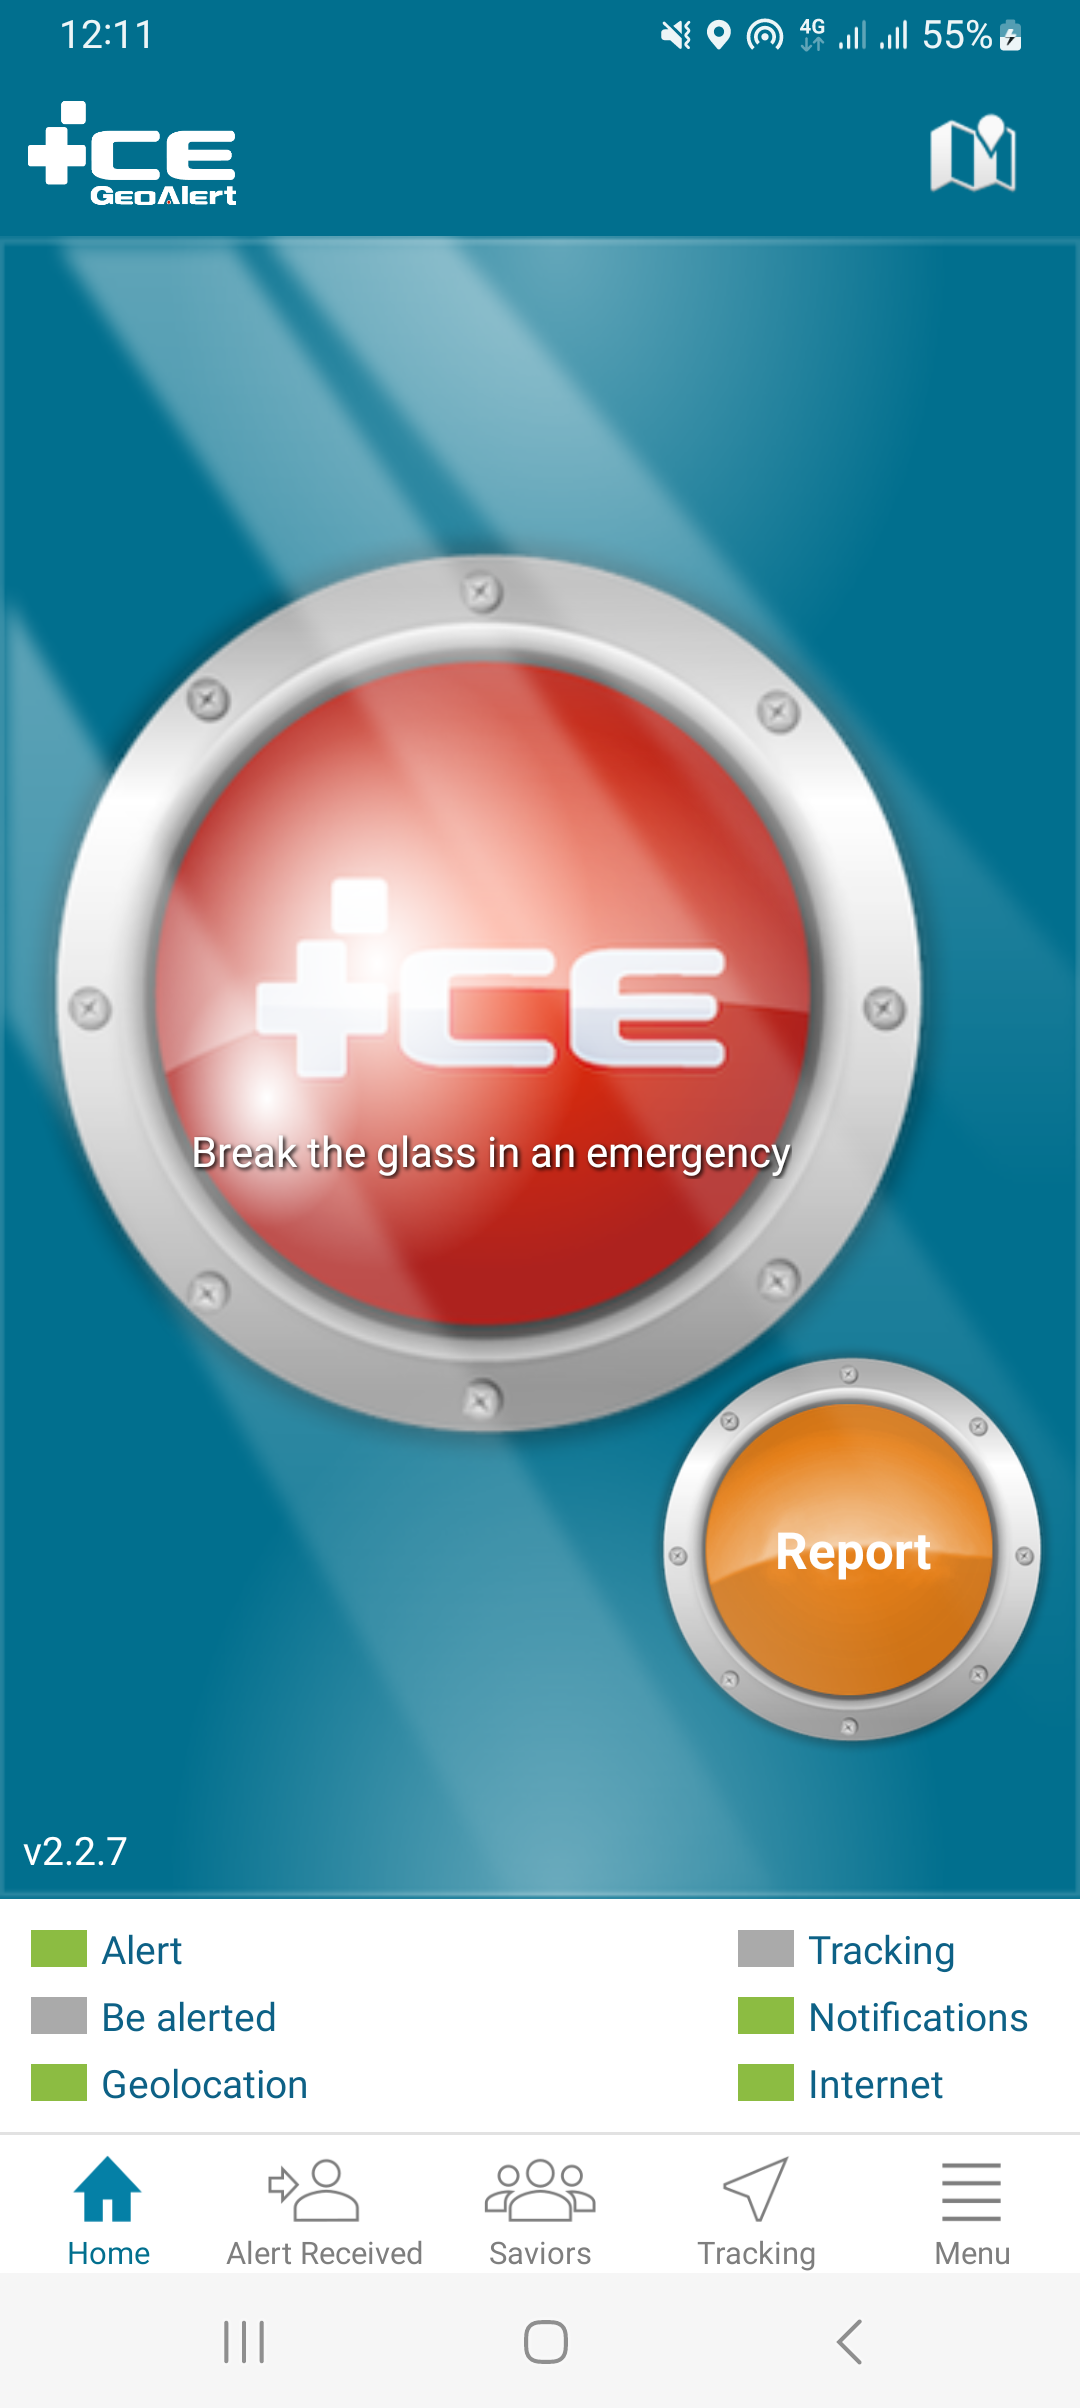
\includegraphics[width=\textwidth]{icegeoalert}
	\caption{Caputre de l’application ICE GeoAlert}
\end{figure}

ICE GeoAlert\footnote{https://icegeoalert.com} est une application qui permet aux utilisateurs d’alerter leurs familles. Pour envoyer un message d’alerte contenant sa géolocalisation à ses proches, la personne en danger doit avoir ICE GeoAlert installé au préalable, et envoie une alerte en cliquant sur le bouton rouge. L’alerte est reçue par message et par email.

\begin{itemize}
	\item Avantages :
	\begin{itemize}
		\item La possibilité d'envoyer rapidement sa géolocalisation aux proches en cas de danger.
		\item Le déclenchement d'une alerte via un bouton dédié, ce qui peut être rapide et intuitif dans une situation d'urgence.
		\item L'alerte est envoyée par message et par e-mail, ce qui garantit que les proches soient informés via plusieurs canaux.
	\end{itemize}
	
	\item Inconvénients :
	\begin{itemize}
		\item Dépendance de la connexion Internet pour envoyer les alertes, ce qui pourrait poser un problème dans des endroits avec une couverture réseau limitée.
		
		\item Nécessité d'une action consciente de la part de la personne en danger pour déclencher l'alerte, ce qui pourrait ne pas être possible dans toutes les situations d'urgence.
	\end{itemize}
	
\end{itemize}

\subsubsection{The Sorority}
\begin{figure}[H]
	\centering
	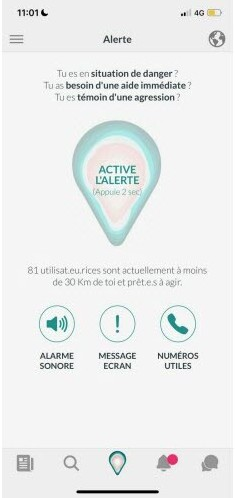
\includegraphics{sorority}
	\caption{Caputre de l’application The Sorority}
\end{figure}

L’application The Sorority\footnote{https://www.jointhesorority.com/} Mise sur l’entraide pour lutter contre le harcèlement de rue… en créant une communauté de femmes et personnes issues des minorités de genre, avec des utilisateurs volontaires et aux profils vérifiés. 

En cas de danger, on peut afficher un message en grand sur l’écran de son smartphone pour interpeller directement les personnes autour, déclencher une alarme sonore pour attirer l’attention et dissuader l’agresseur et également appeler les autorités via un raccourci.

Grâce à la géolocalisation, les cinquante utilisateurs les plus proches sont aussi alertés… L’application permet aussi de trouver un lieu sûr où se réfugier en cas de besoin/danger immédiat. L’application aide aussi à lutter contre les violences conjugales, intra-familiales et contre toutes les formes de harcèlement.

\begin{itemize}
	\item Avantages :
	\begin{itemize}
		\item Encouragement à la solidarité et à l'entraide entre utilisatrices pour lutter contre le harcèlement et les agressions.
		\item Fonctionnalités telles que l'affichage de messages d'urgence,le déclenchement d'alarmes sonores et l'appel aux autorités, qui peuvent dissuader les agresseurs.
		\item Géolocalisation pour alerter les utilisateurs proches en cas de danger, ce qui peut permettre une réponse plus rapide.
	\end{itemize}
	
	\item Inconvénients :
	\begin{itemize}
		\item Limitation à un groupe spécifique d'utilisateurs (femmes et minorités de genre), excluant potentiellement d'autres groupes susceptibles d'être en danger.
		
		\item Dépendance de la participation volontaire des utilisateurs, ce qui pourrait réduire la portée de l'application si le nombre d'utilisateurs n'est pas suffisamment élevé.
	\end{itemize}
	
\end{itemize}

\subsection{Critique de l’existant}

Les applications étudiées visent à répondre à des situations d'urgence cruciales, mais elles présentent des défis significatifs. La dépendance à la connectivité Internet peut s'avérer problématique dans les régions où la couverture réseau est limitée. Une autre limitation importante réside dans la nécessité d'une action manuelle de la part de l'utilisateur en danger pour déclencher une alerte. Dans des scénarios de danger extrême, cette action peut être difficile, voire impossible à réaliser, réduisant ainsi l'utilité de ces applications dans des situations critiques.

De plus, les solutions examinées ont des portées limitées. Certaines applications sont restreintes à des groupes spécifiques d'utilisateurs, excluant potentiellement d'autres personnes en danger.
Dans l'environnement spécifique de Lubumbashi, il est impératif de développer des solutions qui surmontent ces limites pour garantir une protection adéquate et une assistance rapide aux individus en danger.

\subsection{Piste de solution}

La conception d'un système d'appel au secours efficace en cas d'enlèvement à Lubumbashi requiert une approche réfléchie et innovante pour surmonter les limites identifiées dans les applications existantes, telles qu'ICE GeoAlert 2014 et The Sorority. Ce chapitre explore diverses pistes de solutions qui pourraient être envisagées pour répondre aux défis spécifiques de la région.

\begin{itemize}
	\item Alertes automatisées par Reconnaissance Sonore : L'intégration d'un système de reconnaissance sonore sur les smartphones des utilisateurs pourrait permettre la détection automatique de signaux de danger, tels que cris ou bruits suspects. Cette fonctionnalité automatisée renforcerait la réactivité du système, déclenchant des alertes sans nécessiter d'action manuelle de la part de l'utilisateur.
	
	\item Envoi d'Alertes par Différents Canaux : Pour assurer que les alertes soient reçues rapidement, il serait bénéfique d'envisager l'envoi d'alertes par différents canaux. Cela inclut non seulement les réseaux mobiles GSM, mais aussi les applications de messagerie instantanée, les courriels et les notifications push.
\end{itemize}

\section{Conclusion partielle}
Dans ce chapitre, les principales méthodes de localisation des utilisateurs mobiles ont été présentées. On distingue les systèmes de localisation par réseaux terrestres tels que le LORAN C, le GSM ou encore le WIFI qui communiquent avec les équipements mobiles par radio. Ces systèmes qui, malgré leurs limites causées par les obstacles et les conditions météorologiques, sont toujours opérationnels, dans des domaines tels que l’aéronautique, ou en complément des systèmes satellitaires. Nous avons également présenté quelques différents systèmes de localisation satellitaire qui sont le GPS, GLONASS et Galileo. Enfin, nous avons présenté le fonctionnement de localisation d’un terminal mobile grâce aux systèmes satellitaire GPS qui est un système compatible avec la majorité des objets de notre vie quotidienne tels que les smartphones et les véhicules automobiles.
